\documentclass{article}\usepackage[]{graphicx}\usepackage[]{color}
%% maxwidth is the original width if it is less than linewidth
%% otherwise use linewidth (to make sure the graphics do not exceed the margin)
\makeatletter
\def\maxwidth{ %
  \ifdim\Gin@nat@width>\linewidth
    \linewidth
  \else
    \Gin@nat@width
  \fi
}
\makeatother

\definecolor{fgcolor}{rgb}{0.345, 0.345, 0.345}
\newcommand{\hlnum}[1]{\textcolor[rgb]{0.686,0.059,0.569}{#1}}%
\newcommand{\hlstr}[1]{\textcolor[rgb]{0.192,0.494,0.8}{#1}}%
\newcommand{\hlcom}[1]{\textcolor[rgb]{0.678,0.584,0.686}{\textit{#1}}}%
\newcommand{\hlopt}[1]{\textcolor[rgb]{0,0,0}{#1}}%
\newcommand{\hlstd}[1]{\textcolor[rgb]{0.345,0.345,0.345}{#1}}%
\newcommand{\hlkwa}[1]{\textcolor[rgb]{0.161,0.373,0.58}{\textbf{#1}}}%
\newcommand{\hlkwb}[1]{\textcolor[rgb]{0.69,0.353,0.396}{#1}}%
\newcommand{\hlkwc}[1]{\textcolor[rgb]{0.333,0.667,0.333}{#1}}%
\newcommand{\hlkwd}[1]{\textcolor[rgb]{0.737,0.353,0.396}{\textbf{#1}}}%
\let\hlipl\hlkwb

\usepackage{framed}
\makeatletter
\newenvironment{kframe}{%
 \def\at@end@of@kframe{}%
 \ifinner\ifhmode%
  \def\at@end@of@kframe{\end{minipage}}%
  \begin{minipage}{\columnwidth}%
 \fi\fi%
 \def\FrameCommand##1{\hskip\@totalleftmargin \hskip-\fboxsep
 \colorbox{shadecolor}{##1}\hskip-\fboxsep
     % There is no \\@totalrightmargin, so:
     \hskip-\linewidth \hskip-\@totalleftmargin \hskip\columnwidth}%
 \MakeFramed {\advance\hsize-\width
   \@totalleftmargin\z@ \linewidth\hsize
   \@setminipage}}%
 {\par\unskip\endMakeFramed%
 \at@end@of@kframe}
\makeatother

\definecolor{shadecolor}{rgb}{.97, .97, .97}
\definecolor{messagecolor}{rgb}{0, 0, 0}
\definecolor{warningcolor}{rgb}{1, 0, 1}
\definecolor{errorcolor}{rgb}{1, 0, 0}
\newenvironment{knitrout}{}{} % an empty environment to be redefined in TeX

\usepackage{alltt}
\usepackage[sc]{mathpazo}
\renewcommand{\sfdefault}{lmss}
\renewcommand{\ttdefault}{lmtt}
\usepackage[T1]{fontenc}
\usepackage{geometry}
\geometry{verbose,tmargin=2.5cm,bmargin=2.5cm,lmargin=2.5cm,rmargin=2.5cm}
\setcounter{secnumdepth}{2}
\setcounter{tocdepth}{2}
\usepackage[unicode=true,pdfusetitle,
 bookmarks=true,bookmarksnumbered=true,bookmarksopen=true,bookmarksopenlevel=2,
 breaklinks=false,pdfborder={0 0 1},backref=false,colorlinks=false]
 {hyperref}
\hypersetup{
 pdfstartview={XYZ null null 1}}

\makeatletter
%%%%%%%%%%%%%%%%%%%%%%%%%%%%%% User specified LaTeX commands.
\renewcommand{\textfraction}{0.05}
\renewcommand{\topfraction}{0.8}
\renewcommand{\bottomfraction}{0.8}
\renewcommand{\floatpagefraction}{0.75}

\makeatother
\IfFileExists{upquote.sty}{\usepackage{upquote}}{}
\begin{document}








The results below are generated from an R script.

\begin{knitrout}
\definecolor{shadecolor}{rgb}{0.969, 0.969, 0.969}\color{fgcolor}\begin{kframe}
\begin{alltt}
\hlcom{#APPENDIX}
\hlcom{# Jan Domingo}
\hlcom{# May 16, 2019}
\hlcom{#Final: Lab Take-home}

\hlcom{#1}
\hlcom{#(a) What was the longest game streak until a loss?}
\hlstd{p} \hlkwb{=} \hlnum{20}\hlopt{/}\hlnum{38}
\hlstd{n} \hlkwb{=} \hlnum{1000} \hlcom{#Amount of simulations}
\hlstd{gamestreak} \hlkwb{=} \hlkwd{vector}\hlstd{()}
\hlstd{longestStreak} \hlkwb{=} \hlnum{0}

\hlkwa{for} \hlstd{(i} \hlkwa{in} \hlnum{1}\hlopt{:}\hlstd{n) \{}
  \hlstd{streak} \hlkwb{=} \hlnum{0}
  \hlstd{lose} \hlkwb{=} \hlnum{0}
  \hlkwa{while} \hlstd{(lose} \hlopt{==} \hlnum{0}\hlstd{)}
  \hlstd{\{}
    \hlstd{u} \hlkwb{=} \hlkwd{runif}\hlstd{(}\hlnum{1}\hlstd{)}  \hlcom{#runif(1) generates a random number between 0 and 1}
    \hlkwa{if} \hlstd{(u} \hlopt{<} \hlstd{p)}  \hlcom{#If the random number is less than the probability of winning}
      \hlstd{lose} \hlkwb{=} \hlnum{1}  \hlcom{#Stops the simulation if lose = 1}
    \hlstd{streak} \hlkwb{=} \hlstd{streak} \hlopt{+} \hlnum{1}
    \hlkwa{if} \hlstd{(streak} \hlopt{>} \hlstd{longestStreak)}
      \hlstd{longestStreak} \hlkwb{=} \hlstd{streak}
  \hlstd{\}}
  \hlstd{streak}  \hlcom{#Returns the amount of plays until lose}
  \hlstd{longestStreak} \hlcom{#Returns the longest streak in the simulation}

  \hlstd{gamestreak} \hlkwb{=} \hlkwd{c}\hlstd{(gamestreak, streak)}
\hlstd{\}}

\hlcom{#(b) Plot the histogram of game streak lengths}
\hlkwd{hist}\hlstd{(gamestreak,} \hlkwc{br}\hlstd{=}\hlkwd{seq}\hlstd{(}\hlkwd{min}\hlstd{(gamestreak)}\hlopt{-}\hlnum{.5}\hlstd{,} \hlkwd{max}\hlstd{(gamestreak)}\hlopt{+}\hlnum{.5}\hlstd{),} \hlkwc{main} \hlstd{=} \hlstr{"Longest Game Streak per Simulation"}\hlstd{)}
\end{alltt}
\end{kframe}

{\centering 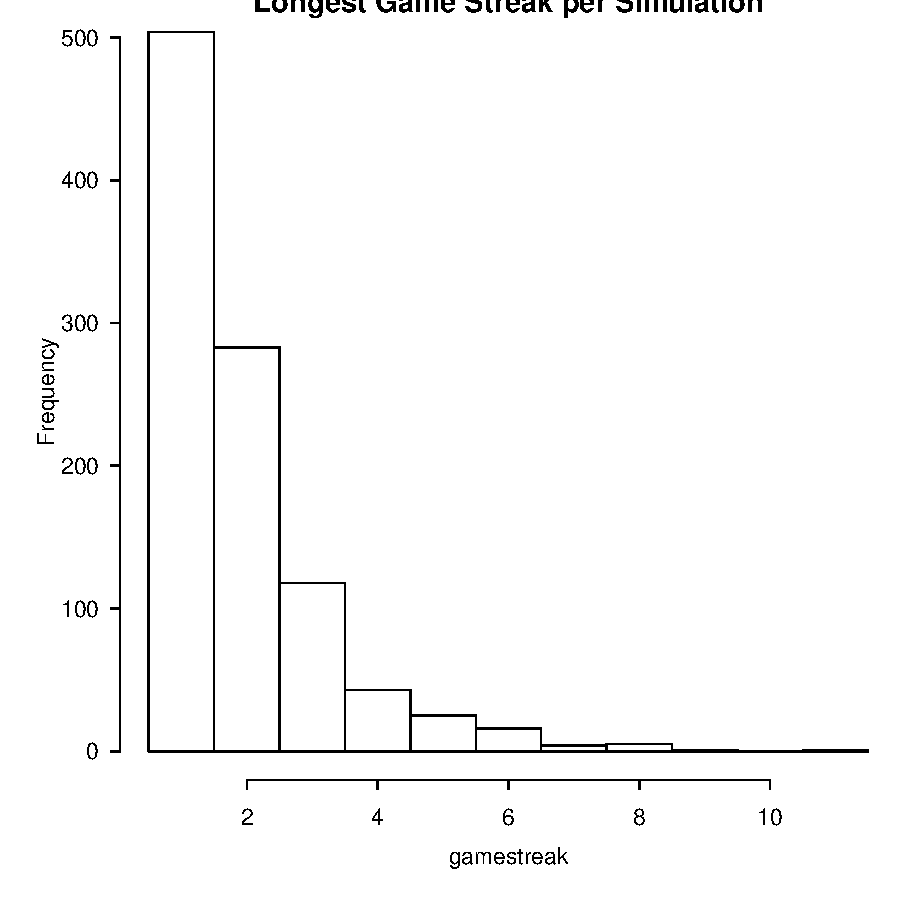
\includegraphics[width=.6\linewidth]{figure/FinalLab-Rnwunnamed-chunk-1-1} 

}


\begin{kframe}\begin{alltt}
\hlcom{#(c) Average of the game streaks}
\hlkwd{mean}\hlstd{(gamestreak)}
\end{alltt}
\begin{verbatim}
## [1] 1.905
\end{verbatim}
\begin{alltt}
\hlcom{#(d) Variance of the game streaks}
\hlkwd{var}\hlstd{(gamestreak)}
\end{alltt}
\begin{verbatim}
## [1] 1.677653
\end{verbatim}
\end{kframe}
\end{knitrout}
\begin{knitrout}
\definecolor{shadecolor}{rgb}{0.969, 0.969, 0.969}\color{fgcolor}\begin{kframe}
\begin{alltt}
\hlcom{#2 }
\hlcom{#(a) What was the longest game streak until 10 black or green spins?}
\hlstd{p} \hlkwb{=} \hlnum{20}\hlopt{/}\hlnum{38}
\hlstd{n} \hlkwb{=} \hlnum{1000}
\hlstd{gamestreak} \hlkwb{=} \hlkwd{vector}\hlstd{()}
\hlstd{longestStreak} \hlkwb{=} \hlnum{0}

\hlkwa{for} \hlstd{(i} \hlkwa{in} \hlnum{1}\hlopt{:}\hlstd{n) \{}
  \hlstd{streak} \hlkwb{=} \hlnum{0}
  \hlstd{lose} \hlkwb{=} \hlnum{0}
  \hlkwa{while} \hlstd{(lose} \hlopt{<=} \hlnum{10}\hlstd{)} \hlcom{#This line is different from #1a. Only stops simulation when lose reaches 10}
  \hlstd{\{}
    \hlstd{u} \hlkwb{=} \hlkwd{runif}\hlstd{(}\hlnum{1}\hlstd{)}  \hlcom{#Generates a random number between 0 and 1}
    \hlkwa{if} \hlstd{(u} \hlopt{<} \hlstd{p)}    \hlcom{#If the random number is less than the proabability of winning}
      \hlstd{lose} \hlkwb{=} \hlstd{lose} \hlopt{+} \hlnum{1} \hlcom{#Then increase the lose count}
    \hlstd{streak} \hlkwb{=} \hlstd{streak} \hlopt{+} \hlnum{1}
    \hlkwa{if} \hlstd{(streak} \hlopt{>} \hlstd{longestStreak)}
      \hlstd{longestStreak} \hlkwb{=} \hlstd{streak}
  \hlstd{\}}
  \hlstd{streak} \hlcom{#Returns the longest streak until 10 black or green spins}
  \hlstd{longestStreak} \hlcom{#Returns the longest streak in the simulation}
  \hlstd{gamestreak} \hlkwb{=} \hlkwd{c}\hlstd{(gamestreak, streak)}
\hlstd{\}}

\hlcom{#(b) Plot a histogram of the game streak lengths}
\hlkwd{hist}\hlstd{(gamestreak,} \hlkwc{br}\hlstd{=}\hlkwd{seq}\hlstd{(}\hlkwd{min}\hlstd{(gamestreak)}\hlopt{-}\hlnum{.5}\hlstd{,} \hlkwd{max}\hlstd{(gamestreak)}\hlopt{+}\hlnum{.5}\hlstd{),} \hlkwc{main} \hlstd{=} \hlstr{"Longest Game Streak per Simulation"}\hlstd{)}
\end{alltt}
\end{kframe}

{\centering 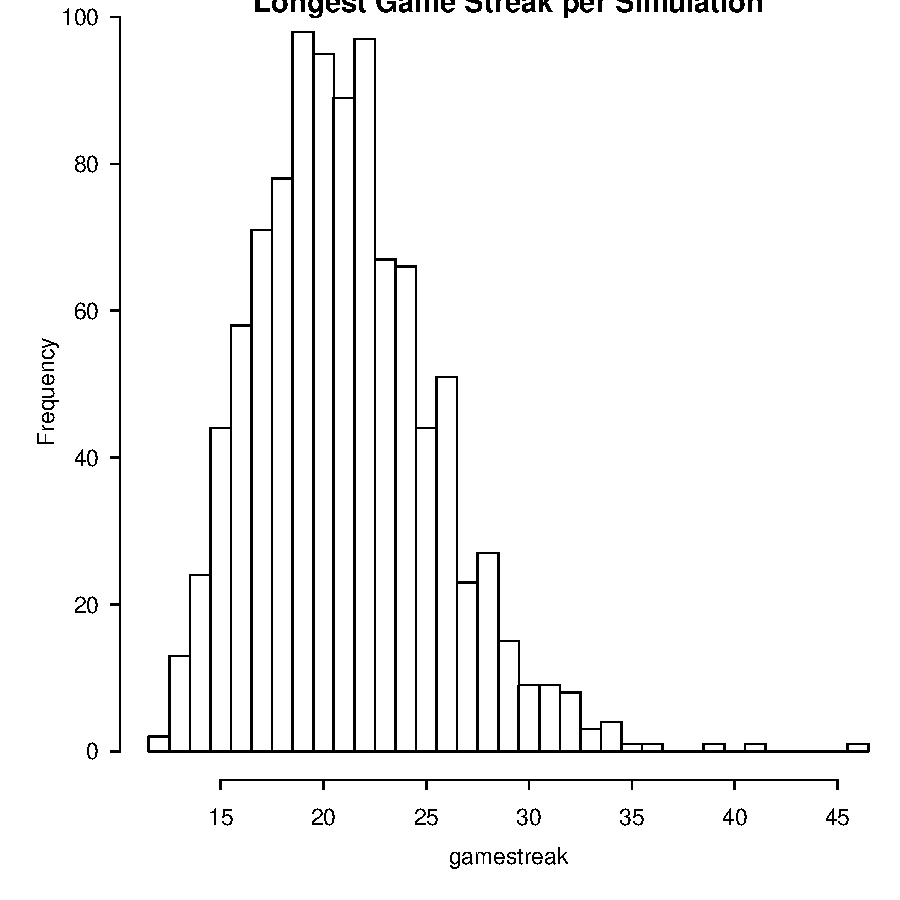
\includegraphics[width=.6\linewidth]{figure/FinalLab-Rnwunnamed-chunk-2-1} 

}


\begin{kframe}\begin{alltt}
\hlcom{#(c) Average of the game streaks}
\hlkwd{mean}\hlstd{(gamestreak)}
\end{alltt}
\begin{verbatim}
## [1] 21.093
\end{verbatim}
\begin{alltt}
\hlcom{#(d) Variance of the game streaks}
\hlkwd{var}\hlstd{(gamestreak)}
\end{alltt}
\begin{verbatim}
## [1] 19.06341
\end{verbatim}
\end{kframe}
\end{knitrout}
\begin{knitrout}
\definecolor{shadecolor}{rgb}{0.969, 0.969, 0.969}\color{fgcolor}\begin{kframe}
\begin{alltt}
\hlcom{#3}
\hlstd{n} \hlkwb{=} \hlnum{10000} \hlcom{#number of variates}
\hlstd{x} \hlkwb{=} \hlnum{1}     \hlcom{#seed value}

\hlkwa{for} \hlstd{(i} \hlkwa{in} \hlnum{1}\hlopt{:}\hlstd{n) \{}
  \hlstd{x} \hlkwb{=} \hlkwd{c}\hlstd{(x, ((}\hlnum{20000}\hlopt{*}\hlstd{x[i])}\hlopt\hlstd{(}\hlnum{2}\hlopt{^}\hlnum{29}\hlopt{-}\hlnum{1}\hlstd{)))} \hlcom{#Linear Congruential Method except with custom a(20000), b(0), and m(2^29) values}
\hlstd{\}}

\hlstd{x} \hlkwb{=} \hlstd{x[}\hlnum{2}\hlopt{:}\hlstd{(n}\hlopt{+}\hlnum{1}\hlstd{)]}  \hlcom{#Disregards seed value, keeps the other 10000 from for loop}
\hlstd{x}
\end{alltt}
\begin{verbatim}
##    [1]     20000 400000000  86555189 231962936 157178049 181796095 232090708  28263494
##    [9] 481681628  20933016 437880331 168319768 214748030 530182911 457727750 369096539
##   [17] 492624661 375132239 410669686 342523522 534486551  94311079 194069657 353324381
##   [25] 192689418 128960842  88983556 480920946 376549435 300431403 505694999 325758582
##   [33] 243135015 260459073 459881478 493983659 174675778  96542123 254664044 523418254
##   [41] 456057322 246533021  37973376 332051846 480621841 300029456 519818664 404959396
##   [49] 490227565 214723318  35942911 524941082 310975395 395266976 452226436 401353294
##   [57] 308889639  19207123 279758635 440936469  87795914 350401030 244598717   6598968
##   [65] 445986805 162784646 107715696 387825068 327308783 108642177 126963183 401121881
##   [73] 512467838 491069010 400625077 240064236  48162927 112125666   3524753 164970659
##   [81] 341431905 176982991  69903777  63687756 297319108 536820675  69021822 141327819
##   [89] 467904496 429941270 300889424   2438601 453638010 178675011  87436384 139122873
##   [97] 392399198   4983002 338921465 434048625 306740041 513790914 109043460  99559518
##  [105] 473022012 237917269  58495807  74424931 292454708 422455566 373793593 481295236
##  [113] 346156681 183222655 309132425  43088924 100667845  90983750 219482621 195851664
##  [121]  23113344  21025629 142656687 201718946 330894746 424071014 470498933 242202903
##  [129] 408700958 159540025 176675927 371074709 327577247 109213067 270474052 506611675
##  [137] 405667608 158952968 246695969  75707910 182230980 339856132 336906740 404866950
##  [145] 251920298 409331176 415869072 177286788 240263756 280466550 103721872 505110807
##  [153] 453078624 265244142  61368409  81277454 440832403 153959558 236485415 412445001
##  [161] 415343396 401185008 164395105 104641036  97908922 210227583 315555959 201621195
##  [169] 523358390 332519144 162905443 376172052 268964157 373482691 168835257 323980721
##  [177] 119395141 437878783 137359768  26908413 223607178   8871370 259999370 392626965
##  [185] 265355714 145324765 413058757 342432443 323519284  17460628 246467850 345166109
##  [193] 236006362 495061399 254639338  29298254 238916099 170872100 258651485 278472515
##  [201] 488340197  48327088 174120200 259271254 325821562 428993193 129831309 318454404
##  [209] 188462807 422344780 305557237 480030998 294329498 337291796  52923285 293134419
##  [217]  58031880 459561329 533454591 393076608 131410227 221430655 501826072 256629766
##  [225] 109410840 467837675 167263092  19193559   8478635 458363035 189894675  68675586
##  [233] 195929662 509331522  41774686 122582484 297100374 457107963 321387492 331293508
##  [241] 346247349 385969922 268481642 386859089 335081579 408868898 297114559 203937052
##  [249] 132729133 292876016 258680990 331701604 455103684 501125817 210173452 306677781
##  [257] 342332736 476862928 283696996 288132552 415552237 283037720 524385327 470164526
##  [265] 533384746  69918430 356747756 477583721 204042399  92185489  95071626 372624149
##  [273] 177864409 518394625 378337679  94960366 294907793  92031754 241597092 103641000
##  [281] 498283540 272950018  96936952  98180379 270658473 436935298  58141653 507537685
##  [289] 135385723 274455827 148345936 170065814 239058815 340837545 100943033 226034640
##  [297] 239729380 330364770  25098323 529029126 467476923 468415846 456393961 536862089
##  [305] 360430911  52498003 377428995 174891340 112814835 365131978 121428578 304429547
##  [313] 474809260  12526232 342795474  67946530 110324259 482606701 268782042 489279068
##  [321]  35265203 392553857 413808447 303846935  96858391 137573112 535692036  44820084
##  [329] 364129541 473783196 429211761 206224021 238081698 125850341 155989232  27776179
##  [337] 399058026  37557074  59075511 394215800 366671965 319526651 158566367  30868723
##  [345] 509783261 486620110   6325392 343175915 160573776 450601309 111067954 324121193
##  [353] 244480586 328333523 202347559  18252882 522291431 468175584 482992160 461769288
##  [361] 132348978 205968770 501770808 225091588 169171265  64818878 371180846 302833603
##  [369] 231313009  43539913 530513269  85565907 310546643 410161552 380390831 355811130
##  [377] 535545606 337445550 443648730 109053903 308419518 280463521  43141872  85886023
##  [385] 270415711 413533497 173556045 250460385 202100370 443181992 437970301 357107035
##  [393] 146970967  51102275 380156367 498369329 378117285 518918565 119719459 481787851
##  [401] 534780283  63371058 405810040 323238413 305620649 137658265  91268392   6742600
##  [409]  97401339 259114892 419807028  16382871 166164290  54860910 390928827 125463107
##  [417] 464372897 128050611 137974530 510988371 429629115 500240356 217693515 384082701
##  [425] 105025412 269236168 444993581 162528353 350564806 298893251 344296926  32215514
##  [433]  65186800 213428092 438097550 217732480  89640879 205608171 269112651 122137225
##  [441] 518725861  23735836 122834676 509102175 286672885 213241431 462973927  65937983
##  [449] 204702584 410983625 178852590 417790918 496372107 162124699 330548471 477892857
##  [457] 481182378 236480325 310645001 229837908  69420018  52184154   6029016 321235936
##  [465] 521398974 335775647 331585212 274747328  72785915 261260279 377874148 488016764
##  [473]  22118020 515640247  51610601 346129058 167633566 449351716 352140771 142809502
##  [481]  36793480 356451930 466643742 447794087 338073609 119926866 334960563 136032542
##  [489] 325933963 529529549 275389614  33604051 455510339  44291241 524687761  76393594
##  [497] 474138205  13199007 376522699 302582314  37371208  99851888 414841991  36761406
##  [505] 251842841 470803909 436142882 315948983   9037530 361973904 310716076  40725175
##  [513]  70328013 495344091   2899317   4281612 269765151 287235361 188472300  75333869
##  [521] 217603734 199075434  74004024 464249284 340145166 212006719 464795833 533706946
##  [529]  71467498 199594918 263136715 325630378 363409570  33006882 323290381 271238827
##  [537] 232855256 286837986 294035965 372211817 521158985 367833846 471697478  53911908
##  [545] 201370712 345536589 129413608  17498069 458416939 194232853 396018915 458620928
##  [553] 515916476 207481491 154548881 211785373 332843121 199994511 201933050 318007458
##  [561] 376348294  35707780 117288370 178389841 289616405  27841221  89285293  73210014
##  [569] 153305703  44287279 445447761 119322866  66120605  99046207 407349321 507216486
##  [577] 153856655 325909059  31449549 315143219 536755771 381554555   7971046 507130344
##  [585]  41629388 437847950  57570679 362346816 252763322  89942024 322928150   5940670
##  [593] 164928669  38502816 183433626 233585137 388943389 145150521 149404223 397840285
##  [601] 378798980 194174879 310280737 460750662 160923596 467679466 224308558  77827684
##  [609] 164909011 182213727 531667043  75596734 106194624  31156084 351423240 287704099
##  [617] 436426813  88988962  52170035 260519927  66348745 366878919 163639363  22186544
##  [625] 275507514 244120407 104075366  58798053 213764910 195135707 199487941 271080359
##  [633] 284720722 361557934  44379741 147204117 419134987 534206557 400011100 308555189
##  [641] 309528966 457716170 137496539  77973858 404034456 245038539 213104392 406548482
##  [649]  59692905 394064847  31966520 454015910 220482257 324347957 484793298 514178251
##  [657] 339590706 397095850 522484488  34348296 308024831 439787186 187585087  47813932
##  [665] 111547509 251544795 415463930 127510453  72232750 472249410 355133688 408478381
##  [673]   2967313 290459790 252542980 514940223   9774287  64728396 172153579 118427757
##  [681] 417551579   4559395 456716041 536011157 521660063 188846537  43881115 375231426
##  [689] 246926042 382200622  44409182 199153206  18831291 279311389  85951045 497113889
##  [697] 502250102 147295190  93111343 358540652 365152684 535548578 396885550  74580865
##  [705] 189909242 360015586 335932579 248999746 517220475 517657763 136612276 109453921
##  [713] 255715853  84761814 334813973 425458008 293091561 274613702  84620470 192288528
##  [721] 164224507 450777413 411922488 165630705 120579130 495338699 431930228 351602010
##  [729] 105007722 452307079 403600561 157073115 230599739 273654510 228133266 336318322
##  [737] 447666992 480528164  37102189  88180998 535888276 211523707 468232231   5319427
##  [745]  88099622 518981009 294857637 162653576 170670251 516638773 157906894 263181498
##  [753] 147548556 328593144  26058449 404196330 261293073 496883237 184177390  76479629
##  [761]  47354561  50932996 215801833 131406471 146310655 266635050 499111948 198111777
##  [769] 128216820 240929064 164853775 151235549 517138337 485510496 362623654 420814212
##  [777] 295839164 465840780 494681417 171192092 216040553  73968272 286080195 170601473
##  [785] 214820595 370870178 531924535 393598535 369402918 177753729 452278269 364271472
##  [793]  91177730 340986244 390568478 434675861 503429088 104695106 105567100 365577948
##  [801] 450894002  59347933 473946690 477866295 486813289 111809015 112955685 497777423
##  [809] 351157327 338153209 101314133 131841886 264676079 511268451 125649094 426016520
##  [817] 189042430 203644738 192029154 345453617  80586341  40345178 523451678  50795500
##  [825] 150236388 398142044 508398959 180996571 347738038 134978906 191179492 532082769
##  [833] 337053069 110221484  37719434  85050045 193853952 334191669 327408961 501589444
##  [841] 355907965 324761962 174958722 386713013  97916134 354467583 508151156  56774770
##  [849]  13423235  29244500 237577921 250857650  94336705 169718746 277020658 442229391
##  [857] 176432186 328092908 221885758 477080585 341869708 343108415 421186509 225586410
##  [865] 401934867 129189597 369116268 350333750 509611450 271625576 451642502 533833336
##  [873] 451783854 139647870 154920978 137532619 262702947 240204954 178168372 155203693
##  [881] 423123509 310880818 114339709 260970051 478894169 106327760   9521529 378277506
##  [889] 502113099  91589745 528222579 442664253 283737610  26670730 301785377 204758538
##  [897] 456321803 167443911 414348093 359348715 420285354 456097384 510902110 315021848
##  [905] 256819415 144294463 208113375 444197928 355595683 521572894  56079270  62066921
##  [913]  92873768 438878851 274496061 416155025 527637678  18933384 173687745 200105830
##  [921] 280829406 381520029 391192868  37573997 397535511 188899001  19419293 228191347
##  [929] 424196500 295864378 433249869 437747371 193474323 257804423 517101667 288981407
##  [937] 212783085 422859414 397689928  56013535 357979654 419481815 491444714 398512323
##  [945] 397786205 370940802 333791802 383132626 430878208 249167539 114984098 263848187
##  [953]  59555781 335939402 385459746 265508951 525710210 124278976 404072981 478667628
##  [961] 407345959 439976486 215488710 311397403 245492400 163518905 297381099 166027942
##  [969]  12255465 296164584 531789848 384213090  28450857 470845251 189241060 418148361
##  [977] 129039353  48590823  80111090 199001576 207456757 196739792  68933281 517991463
##  [985] 368161344  42335635  67273353  68557034 509244217 443158330 501601212  54397054
##  [993] 240614314 312304707 137961426 248908371 300333208 152407732 338478253 159743201
##  [ reached getOption("max.print") -- omitted 9000 entries ]
\end{verbatim}
\begin{alltt}
\hlstd{u} \hlkwb{=} \hlstd{x}\hlopt{/}\hlstd{(}\hlnum{2}\hlopt{^}\hlnum{29}\hlopt{-}\hlnum{1}\hlstd{)}  \hlcom{#Transfrom uniform variates between 0 and 1}

\hlcom{#(a) Plot a histogram of your variates}
\hlkwd{par}\hlstd{(}\hlkwc{mfrow} \hlstd{=} \hlkwd{c}\hlstd{(}\hlnum{2}\hlstd{,}\hlnum{1}\hlstd{))} \hlcom{#2 rows, 1 column for the graph matrix}
\hlkwd{hist}\hlstd{(u,} \hlkwc{main} \hlstd{=}\hlstr{""}\hlstd{,} \hlkwc{xlab}\hlstd{=}\hlstr{"RANDU variiates"}\hlstd{,} \hlkwc{ylab}\hlstd{=}\hlstr{"Frequencies"}\hlstd{)} \hlcom{#Histogram of the n RANDU variates}


\hlcom{#(b) Draw the empirical CDF of oyur variates against the true CDF of a uniform distribution}
\hlkwd{plot.ecdf}\hlstd{(u,} \hlkwc{verticals} \hlstd{=} \hlnum{TRUE}\hlstd{,} \hlkwc{do.p} \hlstd{=} \hlnum{FALSE}\hlstd{,} \hlkwc{xlab} \hlstd{=} \hlstr{"u"}\hlstd{,} \hlkwc{ylab} \hlstd{=} \hlstr{"ECDF"}\hlstd{)}
\hlkwd{abline}\hlstd{(}\hlnum{0}\hlstd{,}\hlnum{1}\hlstd{,} \hlkwc{col}\hlstd{=}\hlstr{"red"}\hlstd{)}
\end{alltt}
\end{kframe}

{\centering 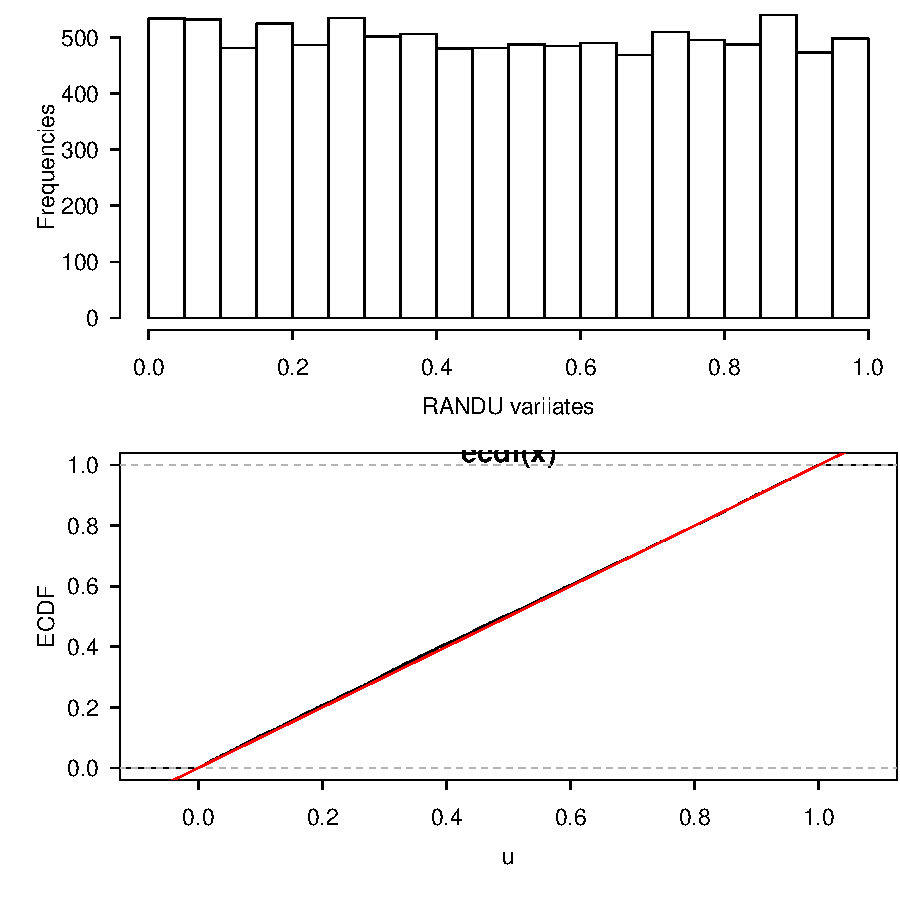
\includegraphics[width=.6\linewidth]{figure/FinalLab-Rnwunnamed-chunk-3-1} 

}


\begin{kframe}\begin{alltt}
\hlcom{#(c)}
\hlkwd{ks.test}\hlstd{(u,} \hlstr{"punif"}\hlstd{,} \hlnum{0}\hlstd{,} \hlnum{1}\hlstd{)} \hlcom{#Komolgorov-smirnov test of RANDU variates against U(0,1)}
\end{alltt}


{\ttfamily\noindent\color{warningcolor}{\#\# Warning in ks.test(u, "{}punif"{}, 0, 1): ties should not be present for the Kolmogorov-Smirnov test}}\begin{verbatim}
## 
## 	One-sample Kolmogorov-Smirnov test
## 
## data:  u
## D = 0.011644, p-value = 0.1328
## alternative hypothesis: two-sided
\end{verbatim}
\end{kframe}
\end{knitrout}
\begin{knitrout}
\definecolor{shadecolor}{rgb}{0.969, 0.969, 0.969}\color{fgcolor}\begin{kframe}
\begin{alltt}
\hlcom{#4}

\hlstd{x1_v} \hlkwb{=} \hlkwd{vector}\hlstd{()}
\hlstd{x2_v} \hlkwb{=} \hlkwd{vector}\hlstd{()}
\hlstd{n} \hlkwb{=} \hlnum{1000}
\hlstd{x_vals} \hlkwb{=} \hlkwd{vector}\hlstd{()}
\hlstd{m} \hlkwb{=} \hlnum{2} \hlcom{#mean}
\hlstd{v} \hlkwb{=} \hlnum{2} \hlcom{#variance}
\hlstd{s} \hlkwb{=} \hlkwd{sqrt}\hlstd{(v)} \hlcom{#standard deviation}

\hlcom{#The following i, ii, and iii are the steps for the Box-Muller Method}
\hlcom{#i Generates two uniform variates}
\hlkwa{for} \hlstd{(i} \hlkwa{in} \hlnum{1}\hlopt{:}\hlstd{n) \{}
  \hlstd{u1} \hlkwb{=} \hlkwd{runif}\hlstd{(}\hlnum{1}\hlstd{)}
  \hlstd{u2} \hlkwb{=} \hlkwd{runif}\hlstd{(}\hlnum{2}\hlstd{)}

\hlcom{#ii Convert Variates to z scores}
\hlstd{z1} \hlkwb{=} \hlkwd{sqrt}\hlstd{(}\hlopt{-}\hlnum{2}\hlopt{*}\hlkwd{log}\hlstd{(u1))}\hlopt{*}\hlkwd{cos}\hlstd{(}\hlnum{2}\hlopt{*}\hlstd{pi}\hlopt{*}\hlstd{u2)}
\hlstd{z2} \hlkwb{=} \hlkwd{sqrt}\hlstd{(}\hlopt{-}\hlnum{2}\hlopt{*}\hlkwd{log}\hlstd{(u1))}\hlopt{*}\hlkwd{sin}\hlstd{(}\hlnum{2}\hlopt{*}\hlstd{pi}\hlopt{*}\hlstd{u2)}

\hlcom{#iii Inverse normal transformation to x variates}
\hlstd{x1} \hlkwb{=} \hlstd{s} \hlopt{*} \hlstd{z1} \hlopt{+} \hlstd{m}
\hlstd{x2} \hlkwb{=} \hlstd{s} \hlopt{*} \hlstd{z2} \hlopt{+} \hlstd{m}

\hlstd{x1_v} \hlkwb{=} \hlkwd{c}\hlstd{(x1_v, x1)}
\hlstd{x2_v} \hlkwb{=} \hlkwd{c}\hlstd{(x2_v, x2)}
\hlstd{\}}

\hlstd{x_vals} \hlkwb{=} \hlkwd{c}\hlstd{(x1_v, x2_v)}

\hlcom{#(a) The mean, variance, and median of the combined variates of x1_v and x2_v}
\hlkwd{mean}\hlstd{(x_vals)}
\end{alltt}
\begin{verbatim}
## [1] 2.013599
\end{verbatim}
\begin{alltt}
\hlkwd{var}\hlstd{(x_vals)}
\end{alltt}
\begin{verbatim}
## [1] 1.971858
\end{verbatim}
\begin{alltt}
\hlkwd{median}\hlstd{(x_vals)}
\end{alltt}
\begin{verbatim}
## [1] 2.001926
\end{verbatim}
\begin{alltt}
\hlcom{#(b) Histogram of these combined variates and an overly with the true density}
\hlstd{x} \hlkwb{<-} \hlkwd{seq}\hlstd{(}\hlopt{-}\hlnum{4}\hlstd{,} \hlnum{8}\hlstd{,} \hlkwc{by}\hlstd{=}\hlnum{0.001}\hlstd{)} \hlcom{#Generate a sequence of numbers from -4 to 8}
\hlstd{y} \hlkwb{<-} \hlkwd{dnorm}\hlstd{(x, m, s)} \hlcom{#Normalize the values with mean=2 and pop sd=sqrt(2)}
\hlkwd{hist}\hlstd{(x_vals,} \hlkwc{freq} \hlstd{=} \hlnum{FALSE}\hlstd{,} \hlkwc{xlab}\hlstd{=}\hlstr{"Normal Variates"}\hlstd{,} \hlkwc{ylim}\hlstd{=}\hlkwd{c}\hlstd{(}\hlnum{0}\hlstd{,}\hlnum{0.30}\hlstd{))}      \hlcom{#Creates histogram with density values}
\hlkwd{lines}\hlstd{(x,y,}\hlkwc{col} \hlstd{=} \hlstr{"red"}\hlstd{)} \hlcom{#Overlay the true density curve over the graph}
\end{alltt}
\end{kframe}

{\centering 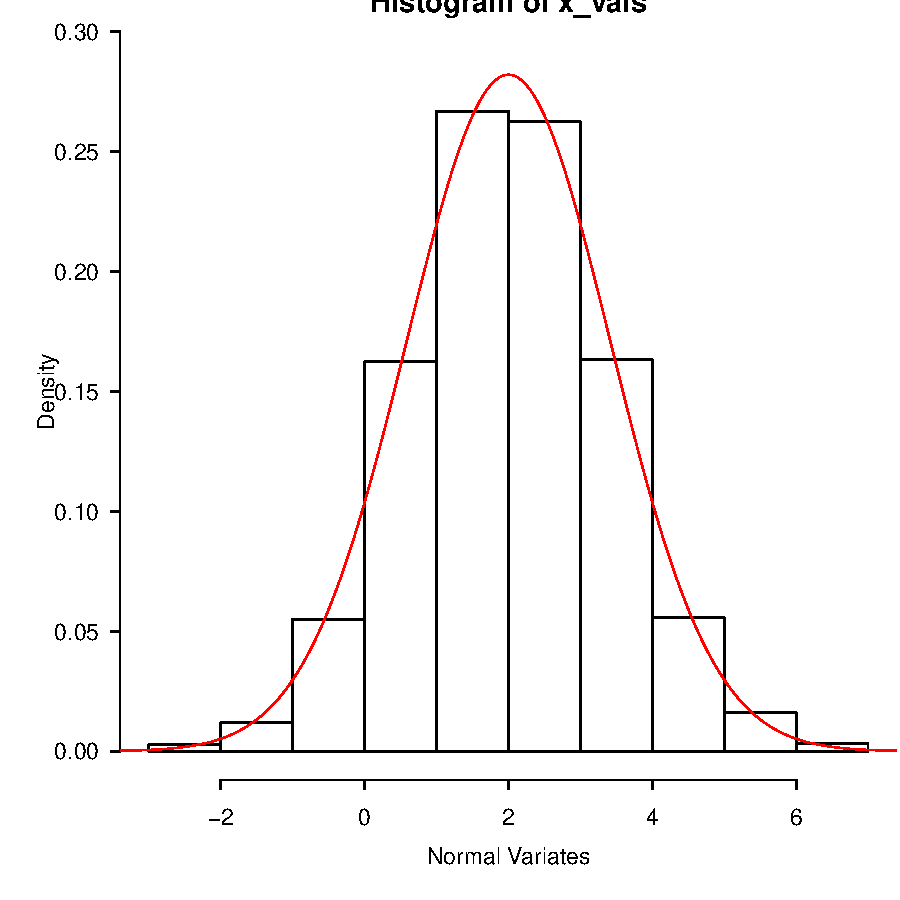
\includegraphics[width=.6\linewidth]{figure/FinalLab-Rnwunnamed-chunk-4-1} 

}


\begin{kframe}\begin{alltt}
\hlcom{#(c) Calculating the empirical rule probabilities}
\hlstd{i} \hlkwb{=} \hlnum{1}
\hlkwd{length}\hlstd{(x_vals[(m}\hlopt{-}\hlstd{i}\hlopt{*}\hlstd{s)} \hlopt{<=} \hlstd{x_vals} \hlopt{&} \hlstd{x_vals} \hlopt{<=} \hlstd{(m}\hlopt{+}\hlstd{i}\hlopt{*}\hlstd{s)])} \hlopt{/} \hlkwd{length}\hlstd{(x_vals)}
\end{alltt}
\begin{verbatim}
## [1] 0.68325
\end{verbatim}
\begin{alltt}
\hlstd{i} \hlkwb{=} \hlnum{2}
\hlkwd{length}\hlstd{(x_vals[(m}\hlopt{-}\hlstd{i}\hlopt{*}\hlstd{s)} \hlopt{<=} \hlstd{x_vals} \hlopt{&} \hlstd{x_vals} \hlopt{<=} \hlstd{(m}\hlopt{+}\hlstd{i}\hlopt{*}\hlstd{s)])} \hlopt{/} \hlkwd{length}\hlstd{(x_vals)}
\end{alltt}
\begin{verbatim}
## [1] 0.954
\end{verbatim}
\begin{alltt}
\hlstd{i} \hlkwb{=} \hlnum{3}
\hlkwd{length}\hlstd{(x_vals[(m}\hlopt{-}\hlstd{i}\hlopt{*}\hlstd{s)} \hlopt{<=} \hlstd{x_vals} \hlopt{&} \hlstd{x_vals} \hlopt{<=} \hlstd{(m}\hlopt{+}\hlstd{i}\hlopt{*}\hlstd{s)])} \hlopt{/} \hlkwd{length}\hlstd{(x_vals)}
\end{alltt}
\begin{verbatim}
## [1] 0.99575
\end{verbatim}
\end{kframe}
\end{knitrout}

The R session information (including the OS info, R version and all
packages used):

\begin{knitrout}
\definecolor{shadecolor}{rgb}{0.969, 0.969, 0.969}\color{fgcolor}\begin{kframe}
\begin{alltt}
\hlkwd{sessionInfo}\hlstd{()}
\end{alltt}
\begin{verbatim}
## R version 3.5.2 (2018-12-20)
## Platform: x86_64-apple-darwin15.6.0 (64-bit)
## Running under: macOS Mojave 10.14.3
## 
## Matrix products: default
## BLAS: /System/Library/Frameworks/Accelerate.framework/Versions/A/Frameworks/vecLib.framework/Versions/A/libBLAS.dylib
## LAPACK: /Library/Frameworks/R.framework/Versions/3.5/Resources/lib/libRlapack.dylib
## 
## locale:
## [1] en_US.UTF-8/en_US.UTF-8/en_US.UTF-8/C/en_US.UTF-8/en_US.UTF-8
## 
## attached base packages:
## [1] stats     graphics  grDevices utils     datasets  methods   base     
## 
## other attached packages:
## [1] knitr_1.22
## 
## loaded via a namespace (and not attached):
## [1] compiler_3.5.2 magrittr_1.5   tools_3.5.2    stringi_1.4.3  highr_0.7     
## [6] stringr_1.4.0  xfun_0.5       evaluate_0.13
\end{verbatim}
\begin{alltt}
\hlkwd{Sys.time}\hlstd{()}
\end{alltt}
\begin{verbatim}
## [1] "2019-05-14 22:48:07 PDT"
\end{verbatim}
\end{kframe}
\end{knitrout}


\end{document}
